

\chapter{Methodology}

To calculate the flux of fireballs from our D6 AllSky Camera, we need to find the total observation area, time, and the total number of events.
In this section, we will describe our methods for finding each of these properties.
We have considered and will discuss obstacles such as camera fish-eye effect and cloud interference.  
Additionally, we will delve into the structure of our database, the fundamental tool for secondary analysis.

\section{Calculating Total Observation Time}

Each night the D6 AllSky camera is placed outside to observe, the Raspberry Pi, the computer behind our observations, runs a program that outputs important information throughout the night.
This output takes on the form of an observation log. 
The observation log is a simple text file that records what processes the camera runs at various times in a given night.
To provide examples, the observation log states when each observation run begins (when the camera is set up initially), when the camera begins its analysis, when a new event is detected, when the analysis goes to sleep, along with many other useful bits of information.

To calculate the total observation time, we can run a Python script that searches for the time associated with a new analysis beginning.  
After this time is recorded, we may continue down the list of information until we find the time associated with that analysis' end.  
By subtracting the two times, we have found the total observation time for that specific night of camera analysis.  
Performing this same method in a loop throughout all of the nights allows us to find how much time we spent observing on a given night. 
By summing up the total time observed over each night, we can attain the total observation time over the course of our data collection period.

A depiction of a simplified observation log and our time analysis table can be seen in Fig. \ref{obslog_time}.
Note that while the information row that contains "New Observation Run Started" sounds as if it represents the start time, we define our start time from the information row that states "A new night has arrived! Frame analysis beginning!".
End times are determined by the information rows labeled "Day has come.  Analysis going to sleep."

\begin{figure}[ht!]
  \centering
  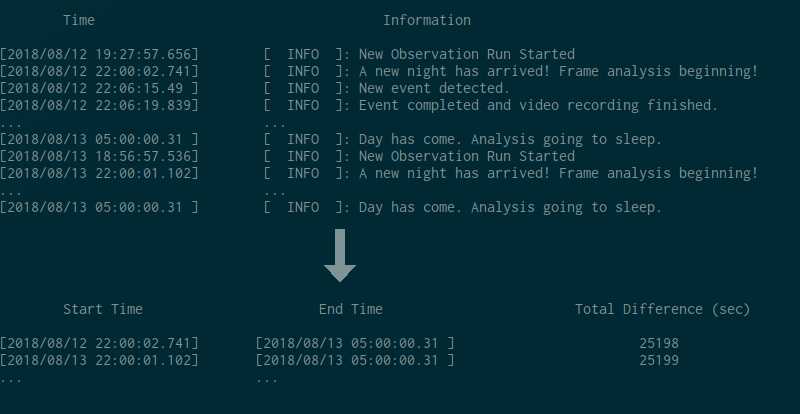
\includegraphics[scale=0.53]{images/obslog_time.png}
  \caption{An example observation log and the resulting time analysis information}
  \label{obslog_time}
\end{figure}

It is imperative that we save not only the total observing time over a given night, but also the start and end times.
This information is crucial for the next section, Calculating Total Observable Area.

\section{Calculating Total Observation Area}

One of the most difficult problems we needed to address for this project was determining the D6 AllSky Camera's observation area.  
In an ideal world, our camera would be able to see all parts of the observable night sky, spanning across all horizons.  
However, due to photometric limitations of our system (and that of most systems), this is not possible. 
Because determining a flux, a primary goal of this project, is directly dependent on observation area, it is vital we get a precise estimate.

To make matters more complicated, our AllSky camera experiences significant fish-eye effects.  
A fish-eye effect refers to the distortion of an image as you travel further from the azimuth (directly overhead).  
For example, imagine a square cloud located directly overhead.  
As that square drifts towards any given horizon, its size becomes smaller relative to you, the observer.  
The significance of this problem as related to our project stems from the fact that while $50\% $ of our camera's pixels may be covered by clouds, this doesn't necessarily mean that $50\%$ of the observable sky is covered.
Therefore, we need some way of relating a given camera region to some observable distance.

To do this, we used observations of the moon and stars to calculate angular distance to pixel ratios for different regions of our camera.
This solution addresses the need to account for a camera fish-eye effect by assigning different regions of view to different observational areas.
By assigning certain pixels with specific angular distance ratios, we can analyze the sky coverage of clouds spanning different camera regions.
To fully understand the methodology behind calculating the total observation area, one must understand how angular separation serves a role in area coverage.

\subsection{Angular Separation}

Consider two objects, visible to you, an observer.
One simple way to compare the two objects is by measuring the distance between them.  
A slightly more complicated way to compare the two would be to imagine two straight lines extending from your line of sight to both objects.  
Because both lines are extending from the same location, we can calculate the associated angle between the two objects, known as the angular separation.
This angular separation may change as you move locations if the objects are nearby. However, if both objects are extremely far away, no small change in observer location will change the angular separation significantly.

We can apply this concept and principle to calculating angular distances between stars and other celestial objects.
By finding the angular separation across a given pixel, we attain a precise estimate for angular coverage of the camera.  
Assuming that the fireballs are passing through our atmosphere at a given height, we can then apply our angular measurements to attain an observational surface area as desired.
It is easy to imagine this surface area used in flux calculations as the base of a cone, where the cone's point represents the viewer's field of view.
Importantly,to calculate angular separation between objects, we need to first have a database of objects to compare.

\subsection{Collecting a Star Catalog}

While the primary aim of the D6 AllSky Camera is to capture video footage of fireballs, it serves many other roles.  
Throughout the night, it takes several snapshots of the nights sky. 
The motivation behind this is primarily to recognize cloud coverage, but these images can store other important information.

Stars are visible in many D6 AllSky Camera's snapshots.  
The first step in creating a catalog of star information is recognizing stars within snapshots.  
We went about this by cleaning the image of hot spots, then enacting a threshold, and using the function \texttt{SimpleBlobDetector} to capture star locations.
All of these processes are performed using Python.

\subsubsection{Hot Pixels and the Dark Frame}

Hot pixels are pixels within a camera that always provide a significant positive photon count, even when the camera is exposed to complete darkness.
These pixels are problematic when trying to locate stars, as they don't represent any real physical object.
Fortunately, this source of error can be accounted for by taking an image while the lens of a camera is covered.  
This is called a dark frame, because the lens is not exposed to light.
The dark frame displays a black image, with a few exceptions, the hot pixels.
By subtracting this dark frame, represented by a 2-dimensional array of values ranging from $0$ to $255$, we are able to remove the hot pixel's effect from all other frames.

\subsubsection{Thresholding}

Once these hot pixels are subtracted from a given frame of interest, the next step is to enact some type of threshold.
In this case, a threshold represents a cutoff photon count for every pixel.  
If a pixel has a count that is lower than the threshold, that photon count is changed to zero, or pure black.  
Alternatively, if a pixel has a count that is higher, the  count becomes 255, or pure white.  
Threshold serves the important role of reducing or simplifying an image.
They also remove some of the inherent error associated with photon counts.
For the purposes of this project, we used an initial threshold of $140$.
The necessary threshold for different images differed in accordance with the amount of surrounding light.
Because of this, if $140$ was not a sufficient threshold, we increased this value in increments of $5$ until the resulting image appeared properly reduced. 
For example, images that contained the moon, a source thats pixels' photon counts bleed into neighboring pixels, needed higher threshold than images without.

\subsubsection{SimpleBlobDetector and Stellarium}

Next, we use the \texttt{SimpleBlobDetector} function from the \texttt{CV2} library to detect potential stars.
This function is able to read an image and scan for objects that meet your specified parameters.
Variable parameters include but are not limited to size (in pixels), circularity, convexity, and color.
In this instance, the color has a value of $255$.  
When enacted, this function scans the picture and returns a list of detected locations centered on the object.
Using simple plotting functions, we can overlay these locations with the original image.

At this point, we have a list of potential object locations, but no foreseeable way of identifying the real ones.
As luck would have it, \textit{Stellarium}, a free astronomy software allows users to view a clear night sky from any point on earth at any time.
Additionally, this interactive software stores information about the stars' names and other important information.
By viewing \textit{Stellarium} and a D6 AllSky Snapshot and comparing the two, we are able to recognize which objects are real and which are false positives.
Because each snapshot is labeled with the corresponding data and time, this method proved sufficient in identifying celestial objects from images.

\begin{figure}[htb]
\centering
  \begin{tabular}{c|c}
    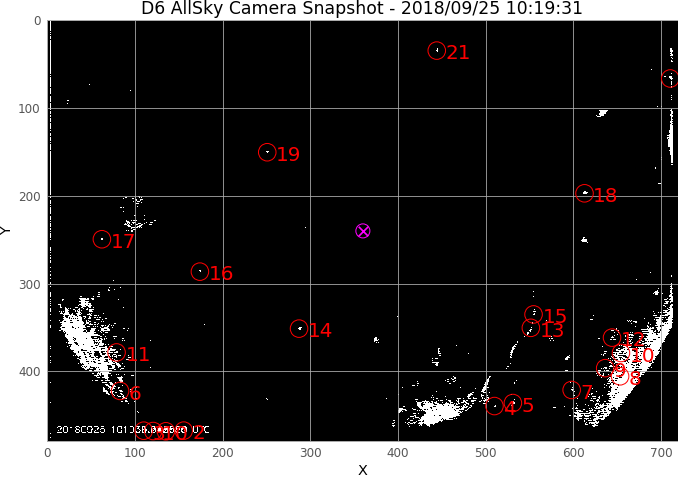
\includegraphics[width=.6\textwidth]{images/FourStarz_OneFrame.png} & 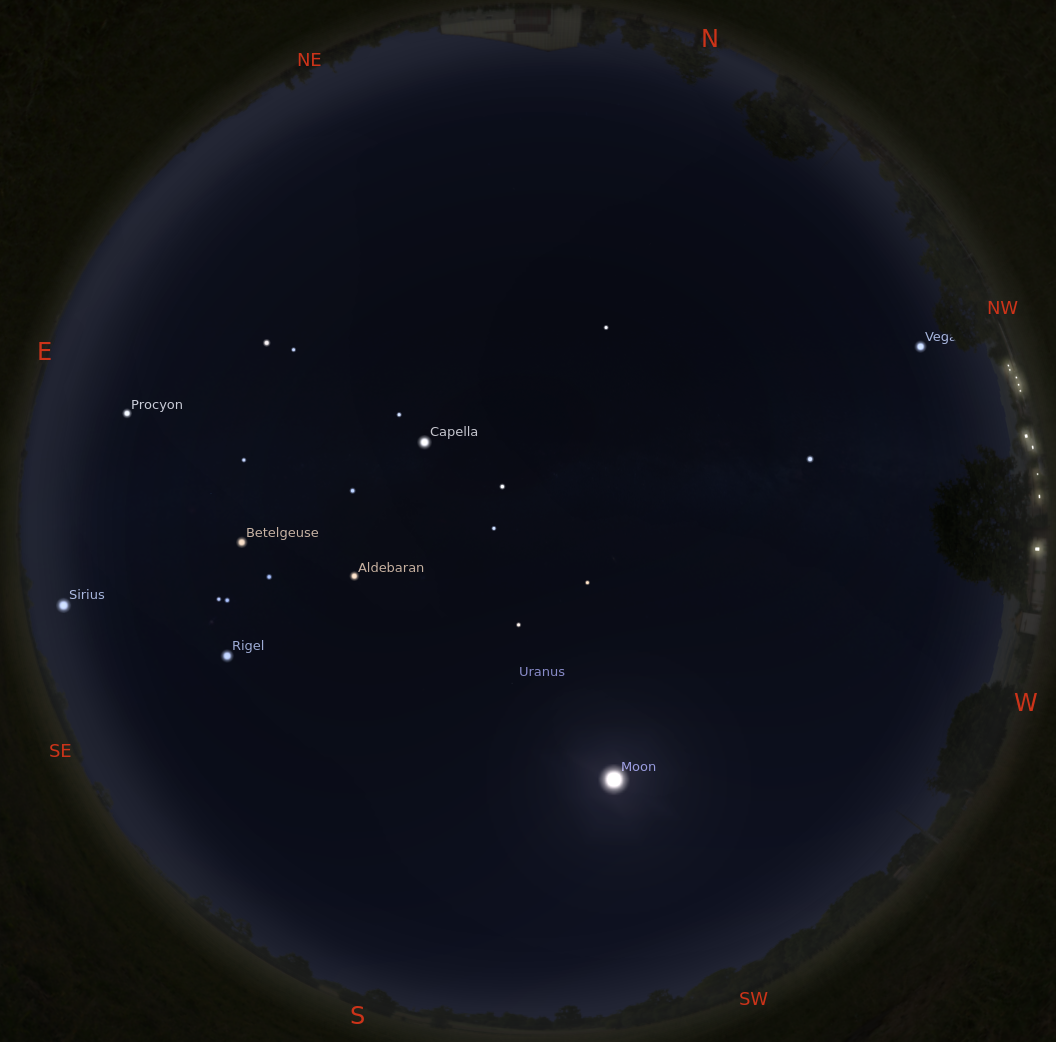
\includegraphics[width=.4\textwidth]{images/zoom_stellarium.png}
  \end{tabular}
 \caption{A D6 AllSky snapshot (left) alongside a Stellarium display (right)}
  \label{star_recognition}
\end{figure}

A depiction of this process can be seen in Fig. \ref{star_recognition}.  
When comparing the two images, it should be clear that the values objects numbered $17$, $16$, $19$, and $21$ correspond to Betelgeuse, Aldebaran, Capella, and Polaris. 
Also note that in the image, there are several recognized objects that don't have any celestial counterpart.
These are all false positives.
Similarly, there are cases in which the \texttt{SimpleBlobDetector} is not able to recognize an object that appears in a snapshot.


Once an object in a given frame was matched to it's name, we used the coding library \texttt{Vizier} to automatically look up the star's right ascension, declination, V-magnitude, azimuth, and elevation.  
This, combined with the star's pixel location, time, and reference file name, was added to our star catalog as a singular data row.

\subsubsection{Azimuth and Elevation}

Each star has several inherent properties such as magnitude, right ascension, and declination.  
The later two represent coordinates that can help locate the star.  
Other properties, such as a star's azimuth and elevation change over time and vary dependent on the observers location.  
These two properties indicate a star's position in the sky relative to an observer and act similarly to spherical coordinates.  

Through finding the azimuth and elevation of a star, we can assign a star a 3-D coordinate value that lays on a unit sphere.  
Using some clever algebra, we can calculate the angular separation between two 3-D coordinates.
A principle of any dot product states that:

$$ \vec{A} \cdot \vec{B} = |\vec{A}||\vec{B}| \cos{(\theta)} $$

where $\theta$ represents the angular separation.  
Because we know that both vectors representing star locations will fall on a unit sphere, their magnitude is $1$.
Using this knowledge, we may transform the above equation to:

$$ \theta = \arccos{(\vec{A} \cdot \vec{B})} $$

Given this formula along with information stored in the star catalog, we are able to calculate angular distance per pixel across different regions of the camera frame.


\subsection{Calculating Angular Areas}

The D6 AllSky camera is a versatile system that's orientation can change slightly from night to night.
Because of this, there are several considerations that must be accounted for when calculating angular distance per pixel across different camera regions.
For example, if pixel $(10,10)$ has an angular separation per pixel of $0.10$ one night, if the camera rotates by $45 \deg$ we may read a different angular separation per pixel at that location.
This is because the pixels may be representing a different area of sky upon rotation.
We have developed a method to account for this consideration.

\subsubsection{Comparing Objects from the same Night}

The star catalog stores information about celestial objects over the course of all observations.
Using constraints from the Time Analysis information (start time, end time, time elapsed), we can isolate rows within the star catalog from a specific night.  
After creating this subsection, we can then use our described method to calculate the angular separation per pixel for every combination of two objects.
One might question where the data behind this angular distance per pixel should be located.
After all, there are two different object locations used to calculate the value.
Our strategy was to locate the point in between the two objects.  
Figure \ref{starcombos} depicts these combinations along with the locations of the angular separation per pixel represented as white dots.

\begin{figure}[ht!]
  \centering
  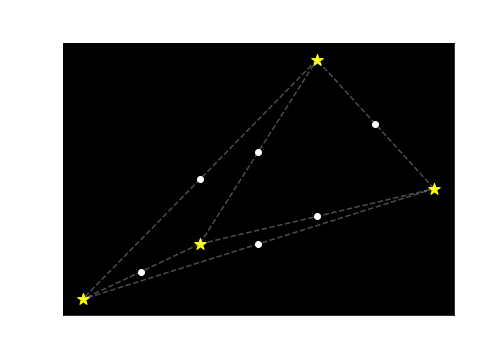
\includegraphics[scale=0.70]{images/star_combinations.png}
  \caption{A simplified depiction of angular distance per pixel locations (white dots) given a set of objects (yellow stars).}
  \label{starcombos}
\end{figure}

Figure \ref{starcombos} gives a general depiction of our method on a much smaller scale.
Note that when comparing objects from this subsection of the star catalog, we are not limited to only comparing different stars.
As an object moves throughout the night sky, its azimuth and elevation change along with its pixel location.
That being said, we can treat each individual row and observation as a unique object, creating many more combinations than if we were to only consider unique stars.

After calculating all potential angular separation per pixel values alongside their location information, we may move on to calculating average angular separation per pixel in different camera regions.
For the sake of simplicity and practicality, we split up our $720 \times 480$ pixel camera frame into $40 \times 40$ pixel squares.  
All angular separation per pixel measurements located inside a given square were averaged over to determine that square's value.
Figure \ref{colorful} shows the resulting average angular separation per pixel for different squares in our camera frame.

\begin{figure}[ht!]
  \centering
  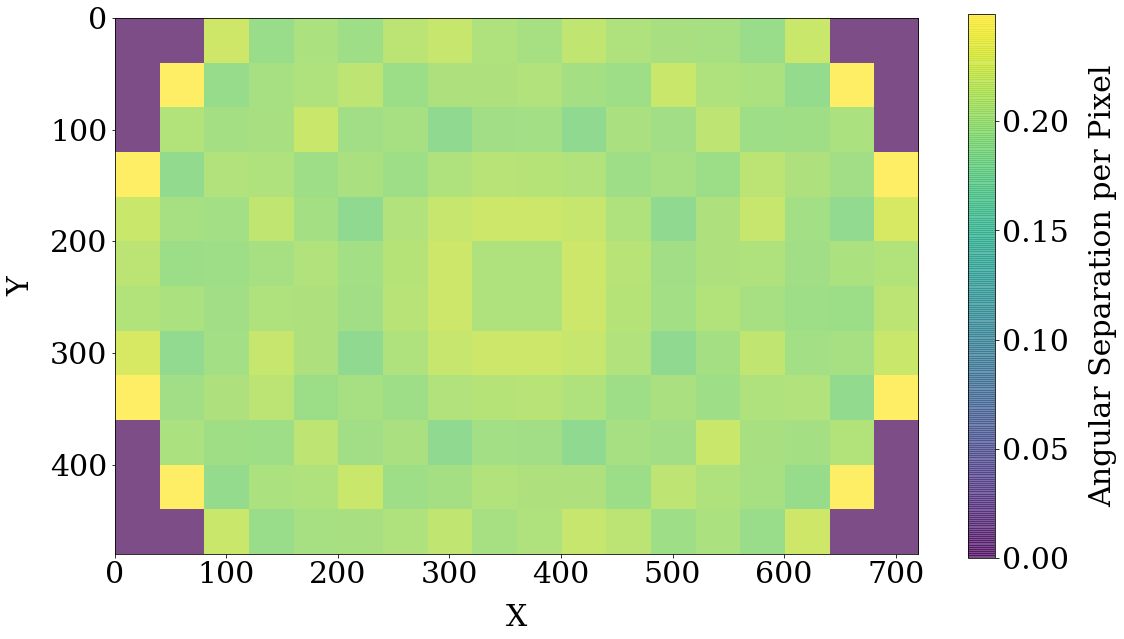
\includegraphics[scale=0.35]{images/boxes_colored.png}
  \caption{Average angular separation per pixel for different camera regions.}
  \label{colorful}
\end{figure}


\section{Calculating Cloud Coverage}

The D6 AllSky Camera does not always remain outside.
For the protection of the system as well as for saving power purposes, the camera is only placed outside during nights where observation conditions are promising.
Some nights, the sky is clear throughout the entire night, while others are partially cloudy.
Because we cannot see or properly analyze fireball events that happen behind clouds, we cannot count cloudy regions as observable areas.
As mentioned previously, the D6 AllSky Camera takes several snapshots of the night sky systematically throughout an observing session.
Specifically, it takes images every $30$ minutes.
By using simple thresholding, we can determine which pixels qualify as not observable areas.
The threshold value that we used in this step was a photon value of $90$.

Unfortunately, some pixels that fall within a broad cloud area are not recognized through this process.
The solution to this problem lies in the \texttt{CV2} functions \texttt{MORPH\_CLOSE} and \texttt{MORPH\_ERODE}.
The first of these functions files in regions of empty space that are next to filled in space.
This is helpful in closing gaps between pixels that represent clouds.
However, because the edges of the clouds are expanded in this process, we must subsequently perform a \texttt{MORPH\_ERODE} that works in the opposite fashion.
Once a hole is completely closed, there is no space within a cloud for the eroding function to open up, hence providing a satisfying answer to the cloud predicament.

After this successful threshold and subsequent closing/eroding process is complete, the next step is implementing the relationships between pixels and angular distance as seen in Fig. \ref{colorful}.
By assigning the correct regional angular separation per pixel value to each pixel within a cloud, we are able to estimate its angular area covered.
Figure \ref{colorclouds} shows the processes taken in calculating the area occupied by clouds.
Note that both a filling and eroding function was used to attain the lower left image.
The observable area during that time is the cloud coverage subtracted from the total observation area.


\begin{figure}[ht!]
  \centering
  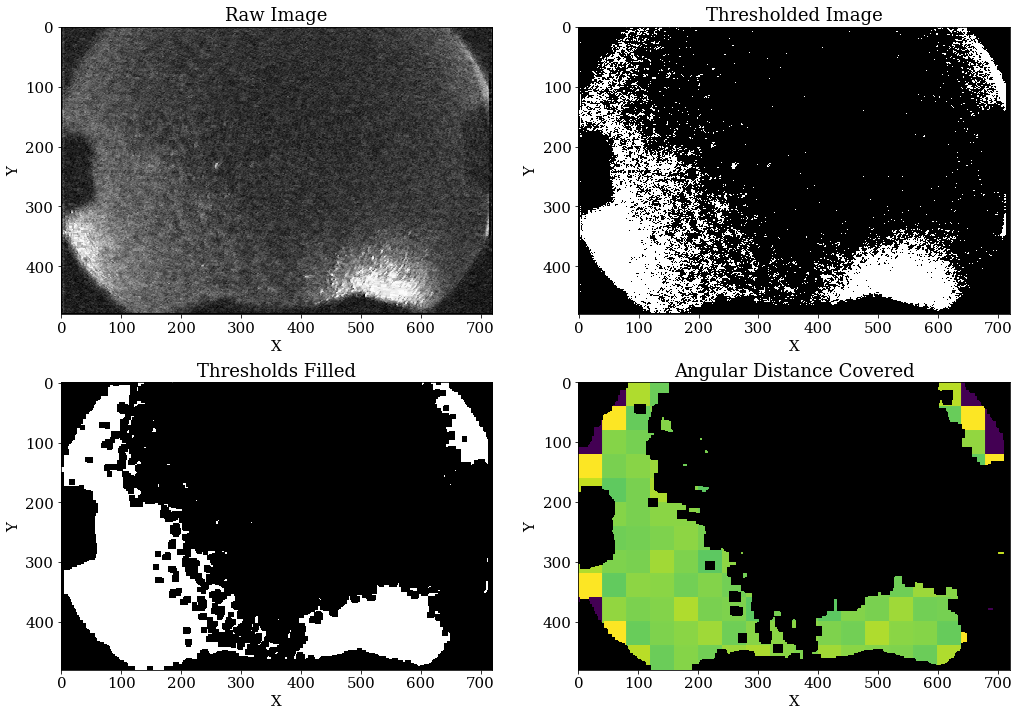
\includegraphics[scale=0.4]{images/Cloud_analysis.png}
  \caption{The processes behind determining the area of cloud coverage.}
  \label{colorcloud}
\end{figure}




This method is performed for each snapshot.
In creating our average area observed calculations, we assume that the sky retains that same amount of cloud coverage for the $15$ minutes prior to and $15$ minutes after the snapshot.
While this isn't precise down to the exact minute, over many observations, the number of over-estimations and under-estimations should cancel and yield an accurate observational area.























 